\documentclass{proposalnsf}
% NSF proposal generation template style file.
% based on latex stylefiles  written by Stefan Llewellyn Smith and
% Sarah Gille, with contributions from other collaborators.
%
% Additions by Ronni Grapenthin, New Mexico Tech.
%
% Obviously it is your responsibility to make sure that everything
% is, in fact, in agreement with the most current NSF Grant 
% Proposal Guide and the respective Program's solicitation! 
% This is all provided `as-is' and no blame or responsibility
% for anything that went wrong will be taken.
%
% Good luck!
%



\usepackage{longtable}
%\usepackage[latin1]{inputenc}
\usepackage[utf8]{inputenc}
\usepackage{latexsym}
\usepackage{amsmath, amsthm, amssymb}
\usepackage{amsfonts}

%\usepackage[pdftex]{graphicx}
\usepackage{graphicx}
\graphicspath{{figures/}}
\usepackage{wrapfig}
\usepackage{adjustbox}
\usepackage{epstopdf}
%\usepackage[
%		 % pdftex,
%	    colorlinks,
%	    pdfstartview=FitH,
%	    linkcolor=black,
%	    citecolor=black,
%	    urlcolor=black,
%	    filecolor=black
%	    ]{hyperref}
\usepackage{url}
\usepackage{lscape}
\usepackage[T1]{fontenc}
\usepackage{floatrow}
\usepackage{enumitem}
\setlist{nosep} % no space before and after
\usepackage{array}
\usepackage{multirow}
\usepackage{ragged2e}
\usepackage{xspace} % custom commands

% color tables
\usepackage{colortbl}
\usepackage{xcolor}

% shaded box
%\usepackage[most]{tcolorbox}
\usepackage{mdframed}

% Tikz
\usepackage{tikz}

% cite
\usepackage{cite}

% highlight
\usepackage{soul}
\usepackage{comment}

% insert PDF
\usepackage{pdfpages}

% itemize
\usepackage{enumitem}



% Insert colors
\input{color_defines}

% Some definitions to make life easier %

\newcommand{\da}{\downarrow}
\newcommand{\la}{\leftarrow}
\newcommand{\ra}{\rightarrow}
\newcommand{\lla}{\longleftarrow}
\newcommand{\llra}{\longleftrightarrow}
\newcommand{\lra}{\longrightarrow}
\newcommand{\Lla}{\Longleftarrow}
\newcommand{\Llra}{\Longleftrightarrow}
\newcommand{\Lra}{\Longrightarrow}
\newcommand{\ua}{\uparrow}

\newcommand{\nea}{\nearrow}
\newcommand{\nwa}{\nwarrow}
\newcommand{\sea}{\searrow}
\newcommand{\swa}{\swarrow}

\newcommand{\mf}{\mathbf}
\newcommand{\mc}{\mathcal}
%\newcommand{\ul}{\underline}
\newcommand{\ol}{\overline}

\newcommand{\eg}{{e.g.,}\xspace}
\newcommand{\viz}{{viz.,}\xspace}
\newcommand{\Eg}{{E.g., }}
\newcommand{\etal}{{et~al.}\xspace}
\newcommand{\ie}{{i.e.,}\xspace}
\newcommand{\etc}{{etc.}}
\newcommand{\ci}{{\it (i) }}
\newcommand{\cii}{{\it (ii) }}
\newcommand{\ciii}{{\it (iii) }}
\newcommand{\civ}{{\it (iv) }}
\newcommand{\cv}{{\it (v) }}
\newcommand{\cvi}{{\it (vi) }}
\newcommand{\cvii}{{\it (vii) }}
\newcommand{\ca}{{\it (a) }}
\newcommand{\cb}{{\it (b) }}
\newcommand{\cc}{{\it (c) }}
\newcommand{\cd}{{\it (d) }}
\newcommand{\ce}{{\it (e) }}
\newcommand{\cf}{{\it (f) }}
\newcommand{\cg}{{\it (g) }}
\newcommand{\ch}{{\it (h) }}
%\newcommand{\ci}{{\it (i) }}
\newcommand{\cj}{{\it (j) }}
\newcommand{\ck}{{\it (k) }}
\newcommand{\cl}{{\it (l) }}
\newcommand{\cm}{{\it (m) }}
\newcommand{\cn}{{\it (n) }}
\newcommand{\co}{{\it (o) }}
\newcommand{\cp}{{\it (p) }}
\newcommand{\cq}{{\it (q) }}
% \newcommand{\note}{{\bf Note: }}

% bold
\newcommand{\cab}{{\it \bfseries (a) }}
\newcommand{\cbb}{{\it \bfseries (b) }}
\newcommand{\ccb}{{\it \bfseries (c) }}
\newcommand{\cdb}{{\it \bfseries (d) }}


% no hyphen in paragaph segmentation
\hyphenpenalty=8000
\exhyphenpenalty=8000
\sloppy

% research task counter
\newcounter{rtaskno}
\newcommand{\rtask}{%
\textbf{TASK~\stepcounter{rtaskno}\thertaskno.}\xspace}

\newcounter{rqno}
\newcommand{\rqs}[1]{\refstepcounter{rqno}\therqno\label{#1}}

%% reference spacing
%\let\OLDthebibliography\thebibliography
%\renewcommand\thebibliography[1]{
%	\OLDthebibliography{#1}
%	\setlength{\parskip}{0pt}
%	\setlength{\itemsep}{0pt plus 0.3ex}
%}

% custom table width
\newcolumntype{L}[1]{>{\raggedright\let\newline\\\arraybackslash\hspace{0pt}}m{#1}}
\newcolumntype{C}[1]{>{\centering\let\newline\\\arraybackslash\hspace{0pt}}m{#1}}
\newcolumntype{R}[1]{>{\raggedleft\let\newline\\\arraybackslash\hspace{0pt}}m{#1}}
\newcolumntype{P}[1]{>{\raggedright\arraybackslash}p{#1}}


% change Figure to Fig.
%\renewcommand{\figurename}{Fig.}

% remove spacing between floats and text
\setlength{\textfloatsep}{0pt}
\setlength{\dbltextfloatsep}{0pt}
\setlength{\intextsep}{0cm}
\setlength{\textfloatsep}{0cm}

% circled text
\newcommand*\circled[1]{\tikz[baseline=(char.base)]{
		\node[shape=circle,fill,inner sep=2pt] (char) {\textcolor{white}{#1}};}}



% paragraph spacing
\makeatletter
\renewcommand\paragraph{\@startsection{paragraph}{4}{\z@}%
                                      {0.3em}%{3.25ex \@plus1ex \@minus.2ex}%
                                      {-1em}%
                                      {\normalfont\normalsize\bfseries}}
\makeatother


%a few commands to highlight issues in the proposal (\TODO, \CHECK, \DummyText)
\RequirePackage{color}
\definecolor{RED}{rgb}{1,0,0}
\definecolor{BLUE}{rgb}{0,0,1}
\definecolor{White}{rgb}{1,1,1}
\providecommand{\TODO}[1]{{\protect\color{red}\noindent {\bf [TODO]}\emph{#1} {\bf [/TODO]}}}
\providecommand{\todo}[1]{{\protect\color{darkred}\noindent {\bf [TODO]}~\emph{#1} \par }}
\providecommand{\CHECK}[1]{{\protect\color{blue} #1 (check) }}
\providecommand{\DummyText}[1]{{\protect\color{white} #1}}

\newcommand{\degrees}{$\!\!$\char23$\!$}

% left alighed bibliography number
\makeatletter
\renewcommand{\@biblabel}[1]{[#1]\hfill}
\makeatother



% Contego
\newcommand{\coolname}{CONTEGO\xspace}
\newcommand{\pve}{\xspace{\relsize{-1.20}\textsc{PASSIVE}}\xspace}
\newcommand{\ave}{\xspace{\relsize{-1.20}\textsc{ACTIVE}}\xspace}


% HYDRA
\newcommand{\coolnameplus}{HYDRA\xspace}
\newcommand{\naive}{SingleCore\xspace}


% HYDRA-C
\newcommand{\pnamemcex}{HYDRA-C\xspace}
\newcommand{\prefname}{HYDRA\xspace}
\newcommand{\prefnamemax}{HYDRA-Tmax\xspace}
\newcommand{\prefnameglobal}{GLOBAL-TMax\xspace}
\newcommand{\prefnamepartition}{HYDRA-TMax\xspace}
\newcommand{\prefnameapa}{APA\xspace}


% SCATE
\newcommand{\pnametee}{SCATE\xspace}
%\newcommand{\pnametz}{\xspace{Contego-TEE}\xspace}
\newcommand{\nw}{\xspace{NW}\xspace}
\newcommand{\sw}{\xspace{SW}\xspace}
\newcommand{\tzignore}{\xspace{IGNORE}\xspace}
\newcommand{\tzfailsafe}{\xspace{FAIL-SAFE}\xspace}

\newcommand{\checkactparam}[3]{\textsf{CheckAct}$($#1$,$ #2$,$ #3$)$}
\newcommand{\checkact}{\textsf{CheckAct}()\xspace}  % this is for dissertation paper name macros 

%%%%%%%%%%%%%%%%%%%%%%%%%%%%%%%%%%%%%%%
%%%%% Document starts here

\begin{document}

%%%%%%%%%%%%%%%%%%%%%%%%%%%%%%%%%%%%%%%
% A - COVER SHEET: Produced by fastlane, type in information there.

\renewcommand{\title}{\noindent {\large{\bf Integrating Security Tasks into Multicore Real-Time Systems}}}
\thispagestyle{empty}

\begin{center}
	\vspace*{1.6in}
	{\title\\}
	\vspace{0.7in}
	{ A Proposal to the\\
		National Science Foundation\\
		\today\\
		Monowar Hasan, Wichita State University		
	}
	
\end{center}
\newpage

%%%%%%%%%%%%%%%%%%%%%%%%%%%%%%%%%%%%%%%
% B - PROJECT SUMMARY

% ============================= %
% NOTE: The Project Summary should be written in the third person, informative to other persons working in the same or related fields, and, insofar as possible, understandable to a scientifically or technically  literate lay reader. It should not be an abstract of the proposal.
% ============================= %

%{\hfil{}\bf\title\hfil{}} \\*[2mm]



\noindent {\large \textbf{Overview}}
\vspace*{1em}

\noindent
TODO

\vspace*{1em}
\noindent {\large \textbf{Intellectual Merit}}
\vspace*{1em}

\noindent
TODO



\vspace*{1em}
\noindent {\large \textbf{Broader Impacts}}
\vspace*{1em}

\noindent
TODO




\pagenumbering{arabic}
\renewcommand{\thepage} {B--\arabic{page}}
\newpage

%%%%%%%%%%%%%%%%%%%%%%%%%%%%%%%%%%%%%%%
% C - TABLE OF CONTENTS: Automatically generated by fastlane.


%%%%%%%%%%%%%%%%%%%%%%%%%%%%%%%%%%%%%%%
% D - PROJECT DESCRIPTION

% reset page numbering to 1.  This is helpful, since the text can only
% be 15 pages (unless otherwise specified, see individual solicitations), 
% and reviewers will want to believe we've kept within those limits

\pagenumbering{arabic}
\renewcommand{\thepage} {D--\arabic{page}}
\newpage

%\title\\

% the main file that contains all PD files

\section{Introduction} \label{sec:intro}

TODO

\paragraph{Research Challanges.}

\subsection{Proposed Research}

In this project we will develop an unified framework that will \textit{integrate monitoring and detection mechanisms into \textbf{multicore} real-time systems} (Section~\ref{sec:proposed_work}). Our techniques will assist the designers of systems to better understand \ca how to \textit{integrate security} into real-time systmes and \cb what are the \textit{trade-offs} on the security front while guaranteeing minimal (or no) perturbations for the real-time properties.

The main outcomes of our research will be to:

\begin{itemize}
	\itemsep 0pt
	\parskip 0pt
	\item Blah
	\item Blah; and
	\item Blah.
\end{itemize}

We will evaluate our proposed techniques using \ca simulations, \cb realistic workloads and embedded benchmark suites (PapaBench~\cite{nemer2006papabench}, MiBench~\cite{guthaus2001mibench},  and  MultiBench~\cite{eembc_multibench}), and \cc off-the-shelf hardware testbeds
(ground rover~\cite{monsterborg} and robotic arm~\cite{robot_arm_rot3u})
[Section~\ref{sec:eval}].  Our research activities described in this proposal will be complemented with tightly integrated educational components reaching from undergraduate/graduate students, students from minority communities, and K-12 students [Section~\ref{sec:broader}]. 


\paragraph{Intellectual Merit.}

\paragraph{Plans for Assessing Success.}




\subsection{Justification for Funding Request}


\paragraph{Foundations for Long-Term Research.} 

The activities proposed here are critical steps for the PI to launch his research career. The proposed work will provide solid foundations for developing security techniques in diverse domains --- from RTS to broader cyber-physical, IoT/edge systems, and even general-purpose computing platforms. While the immediate focus of this research is on integrating security monitoring mechanisms into multicore RTS, the PI believes that the ideas developed in this work can be extended to more general-purpose computing systems and will serve as the basis for future competitive research proposals (\eg NSF CAREER program). Once the proposed ideas have been conceptualized, in Year 3--5, the PI will study the security of hardware/software-based architectures such as real-time hypervisors~\cite{rtzvisor,rt_xen} and TrustZone-enabled RTS~\cite{mukherjee2019optimized,mhasan_iotsnp19}. In Year 5--7, the PI intends to study security/privacy issues of distributed cyber-physical systems such as UAV swarms~\cite{chmaj2015distributed} and vehicular networks~\cite{mhasan_v2x_survey_20}. %software-defined real-time networks~\cite{sdn_qos_rtss17, sdn_qos_infocom21}, and sensor-actuator networks~\cite{van1993sensor,lu2015real}. 
From Year 7 onward, the PI intends to investigate security and resiliency aspects of more general-purpose systems along with IoT/edge-style cyber-physical computing platforms and study emerging technologies such as smart manufacturing, autonomous/electronic vehicles, and robot-aided automation (especially for elderly/disable people). \textbf{Note:} we present the plans beyond Year 2 to show the potentials of our proposed research agenda and the PI's long-term goals.



%\paragraph{Nourishing Collaborative Efforts.}

\paragraph{Strengthening Collaborative Efforts.}

The PI is developing new collaborations with other researchers for interdisciplinary work. In his first nine months as a faculty, the PI has already initiated collaborations with Dr. Sergio Salinas (Wichita State), Dr. Gedare Bloom (U. of Colorado at Colorado Springs), and Dr. Shubhra Kanti (Auburn) on topics related to security and privacy of cyber-physical systems and human-robot interaction. We anticipate leading multiple joint NSF proposals in the future. These projects will not only solve complex, practical problems and  contribute to the growth and development of computing research but also allow the PI to establish a successful academic career.
%academic career. %and lead to joint NSF proposals in the future.

During his PhD, the PI has successfully collaborated with industrial research labs (SRI International and Toyota Motors) that result in multiple publications~\cite{mhasan_sri_17,mhasan_v2x_survey_20} and a patent~\cite{mhasan_sri_patent_1}. The PI intends to strengthen his ties with industrial research and contribute to improving the security of consumer products. Hence, there is a high likelihood that the PI's future research outcomes will be deployed and enhance the security and resiliency of critical cyber-physical systems.


\paragraph{Lack of Support for Seeding Future Research.} 

The PI devotes his career to building secure, trustworthy, and resilient cyber-physical computing platforms. An integral part of the PI's career goals is inspiring, educating, and mentoring the broader community including K-12, undergraduate, and graduate students, and fostering equity and diversity in STEM education. 
%The PI has successful track record of publicly releasing research implementations 
%(refer to the PI's GitHub repositories~\cite{mh_github}) 
% 
The PI intends to promote reproducibility in systems research and disseminate his scientific findings through open-source initiatives. 
 \textbf{The PI \ul{does not have sufficient funds}\footnote{The PI's startup funding supports only one graduate student for 24 months.} to support a doctoral student and initiate these research plans.  The funding support from NSF for the proposed research initiation activities will be one of the significant steps towards achieving the PI's long-term career goals.}

%\todo{talk about collaboration}

%\paragraph{Seeding Career Goals.}




%\subsection{PI's Expertise and Likelihood of Success}

\subsection{PI's Expertise}



The PI, with his diverse research background, is in a unique position to carry out the proposed
research agendas. The PI's research expertise includes \ca real-time and cyber-physical systems security~\cite{mhasan_rtss16,
	mhasan_ecrts17, mhasan_sri_17, mhasan_date18, mhasan_date20, mhasan_resecure_iccps,mhasan_resecure_iot,mhasan_iotsnp19}, \cb development of resilient cyber-physical networks~\cite{sdn_qos_rtss17,sdn_qos_secsdn20,sdn_qos_infocom21}, and \cc resource management in cellular wireless networks~\cite{mhasan_bc15,mhasan_tcom15_1,mhasan_tcom15_2,mhasan_twc14_2,mhasan_twc14_1}. 
%He brings extensive expertise in the design and analysis of resilient real-time cyber-physical systems. 
In recent years, the PI has been at the forefront of the research in real-time security and resiliency with contributions ranging from developing theoretical models~\cite{sdn_qos_infocom21,sdn_qos_rtss17,sdn_qos_secsdn20,mhasan_rtss16,
	mhasan_ecrts17, mhasan_date18, mhasan_date20} as well as designing system architectures~\cite{mhasan_resecure_iccps,mhasan_resecure_iot,mhasan_iotsnp19}. 
	His work on integrating security as a first-class principle of real-time schedulers~\cite{mhasan_rtss16} has won
the \textit{outstanding paper} and \textit{best student paper} awards at the IEEE RTSS. %\footnote{The premier conference in the field of real-time and embedded systems.} 
%The PI  brings extensive expertise in the design and analysis of resilient real-time cyber-physical systems. 
The PI has published his solutions in top real-time and networking conferences/journals including RTSS~\cite{mhasan_rtss16, sdn_qos_rtss17}, ECRTS~\cite{mhasan_ecrts17}, ICCPS~\cite{mhasan_resecure_iccps}, INFOCOM~\cite{sdn_qos_infocom21}, IoT~\cite{mhasan_resecure_iot}, TWC~\cite{mhasan_twc14_1,mhasan_twc14_2}, and Network~\cite{mhasan_network15}. 
%As detailed in Section~\ref{sec:reorder}, the PI has also recently obtained preliminary results, in particular, on developing randomization techniques for single-core real-time systems. 
%The PI also has access to necessary resources (\eg undergraduate/graduate students, hardware, testbed, and research facilities) at Wichita State University to carry out the proposed research agenda (Section~\ref{sec:eval}). 
The \textit{PI has all the resources} (\eg research computers, experimental platforms, and lab facilities) needed to complete this project successfully. 
The PI also has experience working with \textit{underrepresented communities} in computing, most notably \textit{women students} at all levels ---  doctoral, masters, undergraduate, and even middle school students~\cite{mhasan_middleschool_news}. Further, the PI will leverage Wichita State's existing outreach programs 
%\footnote{Supporting letters are attached.} 
(\eg Shocker Engineering Academy~\cite{wsu_sea} and Hub for Cybersecurity Education and Awareness~\cite{wsu_hcea}) as well as resources from other organizations (\eg CRA's undergraduate mentoring programs~\cite{cra_dreu} and NSA's K-12 initiatives~\cite{k12_cybertalk}) and work on broadening participation of high school students and minority communities in engineering.  Hence, the PI is ideal for developing real-time security techniques proposed in this project and fostering diversity in STEM education.





\section{Background and Related Research} \label{sec:background}

\paragraph{Real-Time Systems.} RTS are defined by their strong timing requirements. Some of the common properties and assumptions related to RTS are as follows: 
\ca implemented as a system of periodic tasks, 
\cb worst-case bounds are known for most loops as well as the critical pieces of code, 
%\ciii no dynamically loaded or self-modifying code, 
%\civ recursion is either not used or statically bounded, and
\cc scheduled by priority-driven schemes, and
\cd limited resources (\eg processor, memory, energy). %and
%\cvi stringent timing and safety requirements. 
%The concept of tasks in RTS can be trivially mapped with \textit{processes} or \textit{threads} in general-purpose operating systems (OS).   
%The \textit{scheduler} uses timers and interrupt handlers to enforce timing guarantees
at runtime. 
%This ability of the scheduler to interrupt application processing at precise time instants is essential to ensure the ``correctness'' of the system. 
Each real-time task $\tau_i$  is characterized by $(T_i, C_i, D_i)$ in which $T_i$ is the period (inter-arrival time), $C_i$ is the constant upper bound on the execution time, 
%called worst case execution time (WCET), 
and $D_i$ is the timing constraint (deadline). 
%Tasks in real-time systems are generally characterized by their periods (inter-arrival times), constant, upper bounded execution times,
%%, called worst case execution time (WCET) 
%and temporal constraints (deadlines).
In multicore systems, task scheduling can be viewed as solving an allocation problem 
%(\ie on which processor a task should execute) 
depending on design criteria such as~\cite{mutiprocessor_survey}: \ca \textit{no migration} (tasks are allocated to a fixed core), \cb \textit{task-level migration} (the jobs of a task may execute on different cores), and \cc \textit{job-level migration} (the jobs of a task migrate to and execute on different core although parallel execution of a job is not permitted). Schedulability tests\cite{res_time_1, res_time_rts,  bini2004schedulability,mutiprocessor_survey} are used to determine
if all tasks in the system meet their respective deadlines. If this is the
case, then the task set is deemed to be \textit{``schedulable''} and the system, \textit{safe}.



%\subsection{State-of-the-art}

\paragraph{Related Work.}

Researchers proposed architectural frameworks~\cite{securecore, mohan_s3a, slack_cornell} that use hardware/software mechanisms to
protect against security vulnerabilities. However, those frameworks require custom hardware-support for monitoring, and hence not suitable for legacy or off-the-shelf systems. Integrating monitoring and detection tasks for multicore RTS without custom hardware support is an open research problem. 



%\paragraph{Other Related Research.}

\section{Integrating Monitoring and Detection}

The focus of this proposed research is on integrating or retrofitting security mechanisms into RTS.  When integrating any security mechanisms into RTS, the designers need to ensure that they do not perturb or impact the real-time functions in any significant way while at the same time provide the necessary level of security. This is especially acute in the case of \textit{legacy systems} (\ie existing RTS where modification or perturbation of task parameters such as run-times, periods, and task execution orders is not always feasible.) Any security mechanisms that are introduced not only have to co-exist with existing real-time tasks without violating their real-time and safety constraints but also the {\em parameters of such legacy tasks cannot be adjusted to accommodate the security tasks.}  Not only must the security mechanisms work effectively but they must also not interfere with the deadlines of real-time tasks. For instance, any monitoring and detection mechanism has to be designed so that an adversary cannot easily evade it. This may require that the monitoring and detection tasks be run \textit{frequently}. However, the stringent timing constraints in hard RTS introduce additional complexities for the implementation of such cyber-security mechanisms. For instance, the strict deadlines for the completion of periodic real-time tasks may not allow for frequent execution of security mechanisms. Further, unlike in conventional computing systems, it may not be possible to execute the security mechanisms for arbitrary lengths of time. The challenge is then, how do we develop solutions that address the apparent tension between \textit{security requirements} (\ie having enough cycles for effective monitoring detection) and the \textit{timing and safety requirements} (\ie not interfere with deadlines)?



\begin{wraptable}{r}{0.510\textwidth}
%\begin{table*}% [h]
%\renewcommand{\arraystretch}{1.3}
%\vspace{-\baselineskip}

\caption{Example of security tasks --- this is by no stretch meant to be an exhaustive list.}
\label{table:rtos}
%\centering
%\scriptsize
\small
\vspace{2mm}
\begin{tabular}{P{4.0cm}||P{3.35cm}}
    \hline %\\
    \bfseries Security Task & \bfseries Approach/Tools\\
    \hline\hline
    File-system checking & Tripwire~\cite{tripwire}, AIDE~\cite{aide} \\
    Network packet monitoring & Bro~\cite{bro}, Snort~\cite{snort} \\
    Hardware event monitoring & perf~\cite{linux_perf}, OProfile~\cite{oprofile}\\ 
    Application specific checks & Behavior-based detection~\cite{anomaly_detection_survey, securecore,securecore_memory,securecore_syscal} \\
    \hline
    \end{tabular}
%\end{table*}
%\vspace*{0.1\baselineskip}
\vspace{-2mm}
\end{wraptable} 



Hence, we propose to improve the security posture of RTS through integration of \textit{\textbf{``security tasks''}} (\ie tasks that are specific for intrusion monitoring and detection tasks purposes) while ensuring that the existing real-time tasks are \textit{not affected} by such integration. Security tasks could include protection, detection or response mechanisms, depending on the system requirements --- for instance, a sensor correlation task (to detect sensor manipulation) or an anomaly detection task (that checks possible intrusions)~\cite{caml_song2016}. Table~\ref{table:rtos} presents some examples of security tasks that can be integrated into legacy systems. \textbf{Note:} Table~\ref{table:rtos} is by no stretch meant to be an exhaustive list. Our proposed work will \textit{not} design towards any specific security mechanisms --- our focus here is to \textit{integrate any designer-provided security monitoring tasks} and \textit{schedule} them with respect to real-time constraints into a multicore RTS.


\paragraph{Considerations  for Integrating Security  Mechanisms.} To begin with, we propose the following two performance criteria:

\begin{enumerate}[leftmargin=0.2in]
	\item \textit{Monitoring Frequency:} In order to provide the best protection, the security tasks need to be executed quite often. On the one hand, if the interval between consecutive monitoring events is too large, the adversary may harm the system (and remain undetected) between two invocations of the security task. On the other hand, if the security tasks are executed very frequently then it may impact the schedulability of the real-time tasks. Herein lies an important \textit{trade-off} between \textit{monitoring frequency} and \textit{schedulability}. 
	
	\item \textit{Responsiveness:} In some circumstances, a security task may need to execute with less interference from higher-priority tasks. For instance, consider the scenario where a security breach is suspected. In such an event the security task may be required to \textit{perform more fine-grained checking instead of waiting for its next periodic slot}. This may result in delayed execution of low-priority, non-critical, real-time tasks.
	However, the scheduling policy needs to ensure that the system remains secure without violating real-time constraints for critical, high-priority, real-time tasks. 
	
	%	\item \textit{Atomicity:} Depending on the operation, some of the security tasks may need to be executed \textit{without preemption}. For instance, let us consider a security task that scans the process table and has been preempted in the middle of its operation. An adversary may corrupt the process table entry that has already been scanned before the next scheduling point of the security task. When the security tasks are rescheduled, it will start scanning from its last known state and may not be able to detect the changes in a timely manner.  
\end{enumerate}

%Unlike single core systems, integrating security into multicore platforms is more challenging since designers have multiple choices across cores to retrofit security mechanisms. 
Unlike single core systems, integrating security into multicore platforms is more challenging since the designers now have multiple choices for where to allocate the security tasks. For instance, should the engineers: 
\ci \textit{dedicate a core} to all the security tasks; or 
\cii \textit{spread the security tasks to all cores} (in conjunction with the real-time tasks) and if so, how to determine the \textit{task-to-core assignment}? or \ciii \textit{execute them continuously} across any available core? In addition, how the designers can \textit{determine the monitoring frequency of security tasks}? How do we develop a \textit{reactive framework that dynamically adjust security tasks into available cores for better responsiveness upon suspicion of a security breach?} These are themselves critical research challenges that need to be investigated.

\paragraph{Adversary Model.}

We assume that an adversary may destabilize the system by leveraging (known) vulnerabilities. 
%For example, an attacker could compromise the file system (resulting in corrupted information/system log), change the of control/actuation commands or infer side-channel information (\eg user tasks, cache, thermal profiles) to launch further attacks (\eg denial of service). 
%While there exists mechanisms (such as Simplex~\cite{sha2001using,l1_simplex}) that guarantee (hardware/software) fault tolerance, I consider the cases where an attacker intentionally induces faults (\ie adversarial artifacts) that may jeopardize the safety of the system (\eg results in miss deadlines). 
Our focus is on threats that can be dealt with by \textit{integrating additional security tasks} into the host (see Table~\ref{table:rtos} for related examples). The addition of such tasks may necessitate changing the schedule or increasing the execution time of real-time tasks as was the case in earlier work~\cite{sibin_RT_security_journal,sg1, sg1, lin2009static,xie2007improving, zhang2013design, jiang2013optimization}.  In this research we consider situations where additional security tasks  are only allowed to have no (or minimal) impact on the schedule of existing real-time tasks and are not allowed to modify real-time parameters. We note that the design of integration techniques and the design of the specific security tasks are orthogonal problems; and our proposed techniques are agnostic to the specific monitoring mechanism. 

%Since we aim to maximize the frequency of execution of security tasks, mechanisms whose performance improves with frequency of execution (\eg intrusion monitoring and detection tasks or logging/tracing mechanisms) benefit from my model.



%For instance,is it better to \textit{dedicate a core} to all the security tasks or is it better to \textit{spread them out} (in conjunction with the real-time tasks) and if so, to \textit{which cores}? It is not trivial to determine the execution frequency and core assignment of security mechanisms (\ie \textit{what} security tasks will execute on \textit{which core} and with \textit{what frequency}). This in itself a research challenge that needs to be investigated.

\paragraph{Preliminary Work: Contego~\cite{mhasan_rtss16, mhasan_ecrts17} and Hydra~\cite{mhasan_date18, mhasan_date20}.}

The PI's dissertation work~\cite{mhasan_rtss16, mhasan_ecrts17, mhasan_date18, mhasan_date20} provides the foundation of this research. 



%Unlike single core systems, integrating security into multicore platforms is more challenging since the designers now have multiple choices for where to allocate the security tasks. For instance, should the engineers: 
%%\ci \textit{dedicate a core} to all the security tasks; or 
%\ci \textit{spread the security tasks to all cores} (in conjunction with the real-time tasks) and if so, how to determine the \textit{task-to-core assignment}? or \ciii \textit{execute them continuously} across any available core? In addition, how the designers can \textit{determine the periods of the security tasks}?
%Chapter~\ref{ch:hydra-c} addresses aforementioned issues. 


In particular, I first develop
a low-complexity iterative solution (called \coolnameplus) that
jointly finds the security tasks’ periods and core assignments. The \coolnameplus mechanism assumes that the security tasks are \textit{statically assigned} across all available cores. 
%I compare \coolnameplus with another scheme that allocates a dedicated core for security tasks while the real-time tasks are assigned to the remaining cores. I find out on average, \coolnameplus can provide 27.23\% faster intrusion detection rate (on a quad core system) when compared to the other scheme. 
%In Chapter~\ref{ch:hydra-c} 
I then extend \coolnameplus with an alternate design mechanism, \pnamemcex, that \textit{can raise the ``responsiveness'' of monitoring tasks by increasing their frequency of execution}. The key intuition is that if the security tasks are able to execute with as few interruptions as possible (\eg by moving immediately to an empty core when they are interrupted), then there is much higher chance of successful detection and correspondingly, a much lower chance of successful adversarial action. 
%I therefore present a design-time framework (named \pnamemcex) that 
%\pnamemcex enables \textit{continuous execution} of security tasks (\ie execute as frequently as possible) across cores, without impacting timing requirements of existing real-time tasks. 
\pnamemcex provides better monitoring when compared to \coolnameplus but comes with a cost (in terms of context switch overhead).


\section{Evaluation} \label{sec:eval}

We will evaluate our proposed schemes using a variety of methods as we present below. 
%The evaluation process will demonstrate the feasibility of our research results. 
Our implementation details and source code will be \textit{\ul{publicly available}}.



\paragraph{Simulation-based Evaluation.} All of our approaches will first be evaluated using an \textit{internally developed simulator}. We will use the simulator 
%to analyze the scalability of the algorithms and also 
to test with a more diverse set of real-time task parameters to explore the design-space and scalability of the solutions/algorithms that have been developed. In the past, we extensively use open-source and custom in-house simulators~\cite{sdn_qos_rtss17, sdn_qos_infocom21, sdn_qos_secsdn20, mhasan_rtss16, mhasan_certs16, mhasan_date18, mhasan_twc14_1, mhasan_twc14_2, mhasan_tcom15_1, mhasan_tcom15_2} primarily to test the theories, and we will use similar techniques to evaluate our proposed schemes. 




\paragraph{System Integration and Benchmarks.} We will integrate our proposed ideas into \textit{two real-time kernels} (RT\_PREEMPT~\cite{rt_patch} and LITMUS\textsuperscript{RT}~\cite{litmus_rt}) and use OP-TEE~\cite{optee} as our secure enclave. We will develop kernel patches and evaluate them on both x86 (UP Extreme~\cite{up_extreme}) and ARM (Raspberry Pi~\cite{rpi4}) embedded hardware platforms. We will use existing intrusion detection tools such as Tripwire~\cite{tripwire}, AIDE~\cite{aide}, and Bro~\cite{bro} as security tasks. Further, we will evaluate the efficacy of our scheduler implementations using \textit{three embedded benchmark suites}: PapaBench~\cite{nemer2006papabench}, MiBench~\cite{guthaus2001mibench},  and MultiBench~\cite{eembc_multibench}. These tools and benchmarks will enable us to evaluate the performance of models with realistic workloads. We will use \textit{multiple performance indicators} (such as context switch and memory overheads, scheduling delays) to evaluate the trade-offs of integrating security into existing real-time schedulers.


\begin{wrapfigure}{r}{0.350\textwidth}
	\centering
		\vspace*{-0.3\baselineskip}
%	\hspace*{-1.5em}
	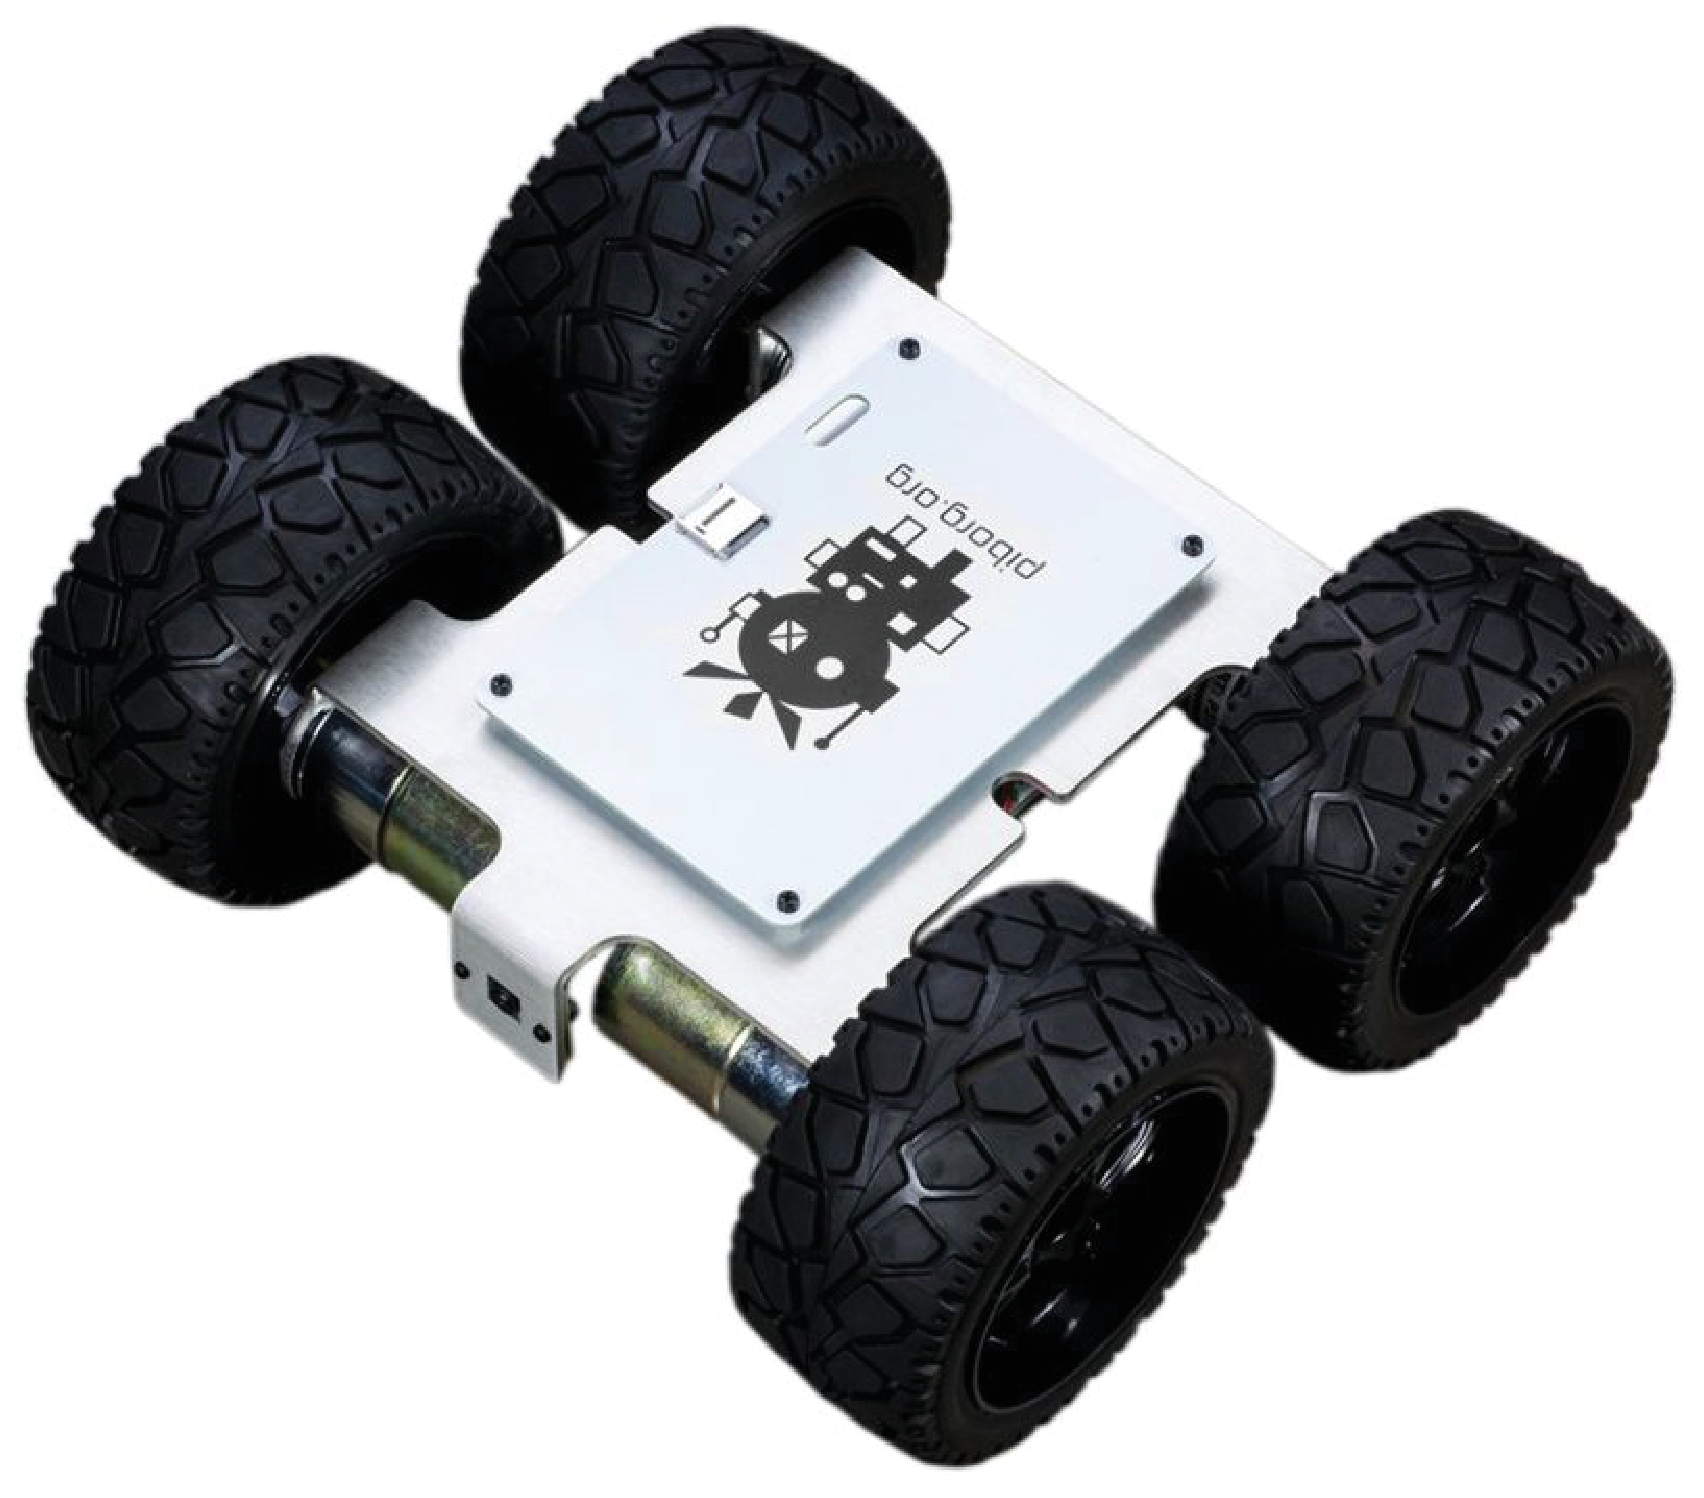
\includegraphics[scale=0.10]{piborg}
	\hspace*{1em}
	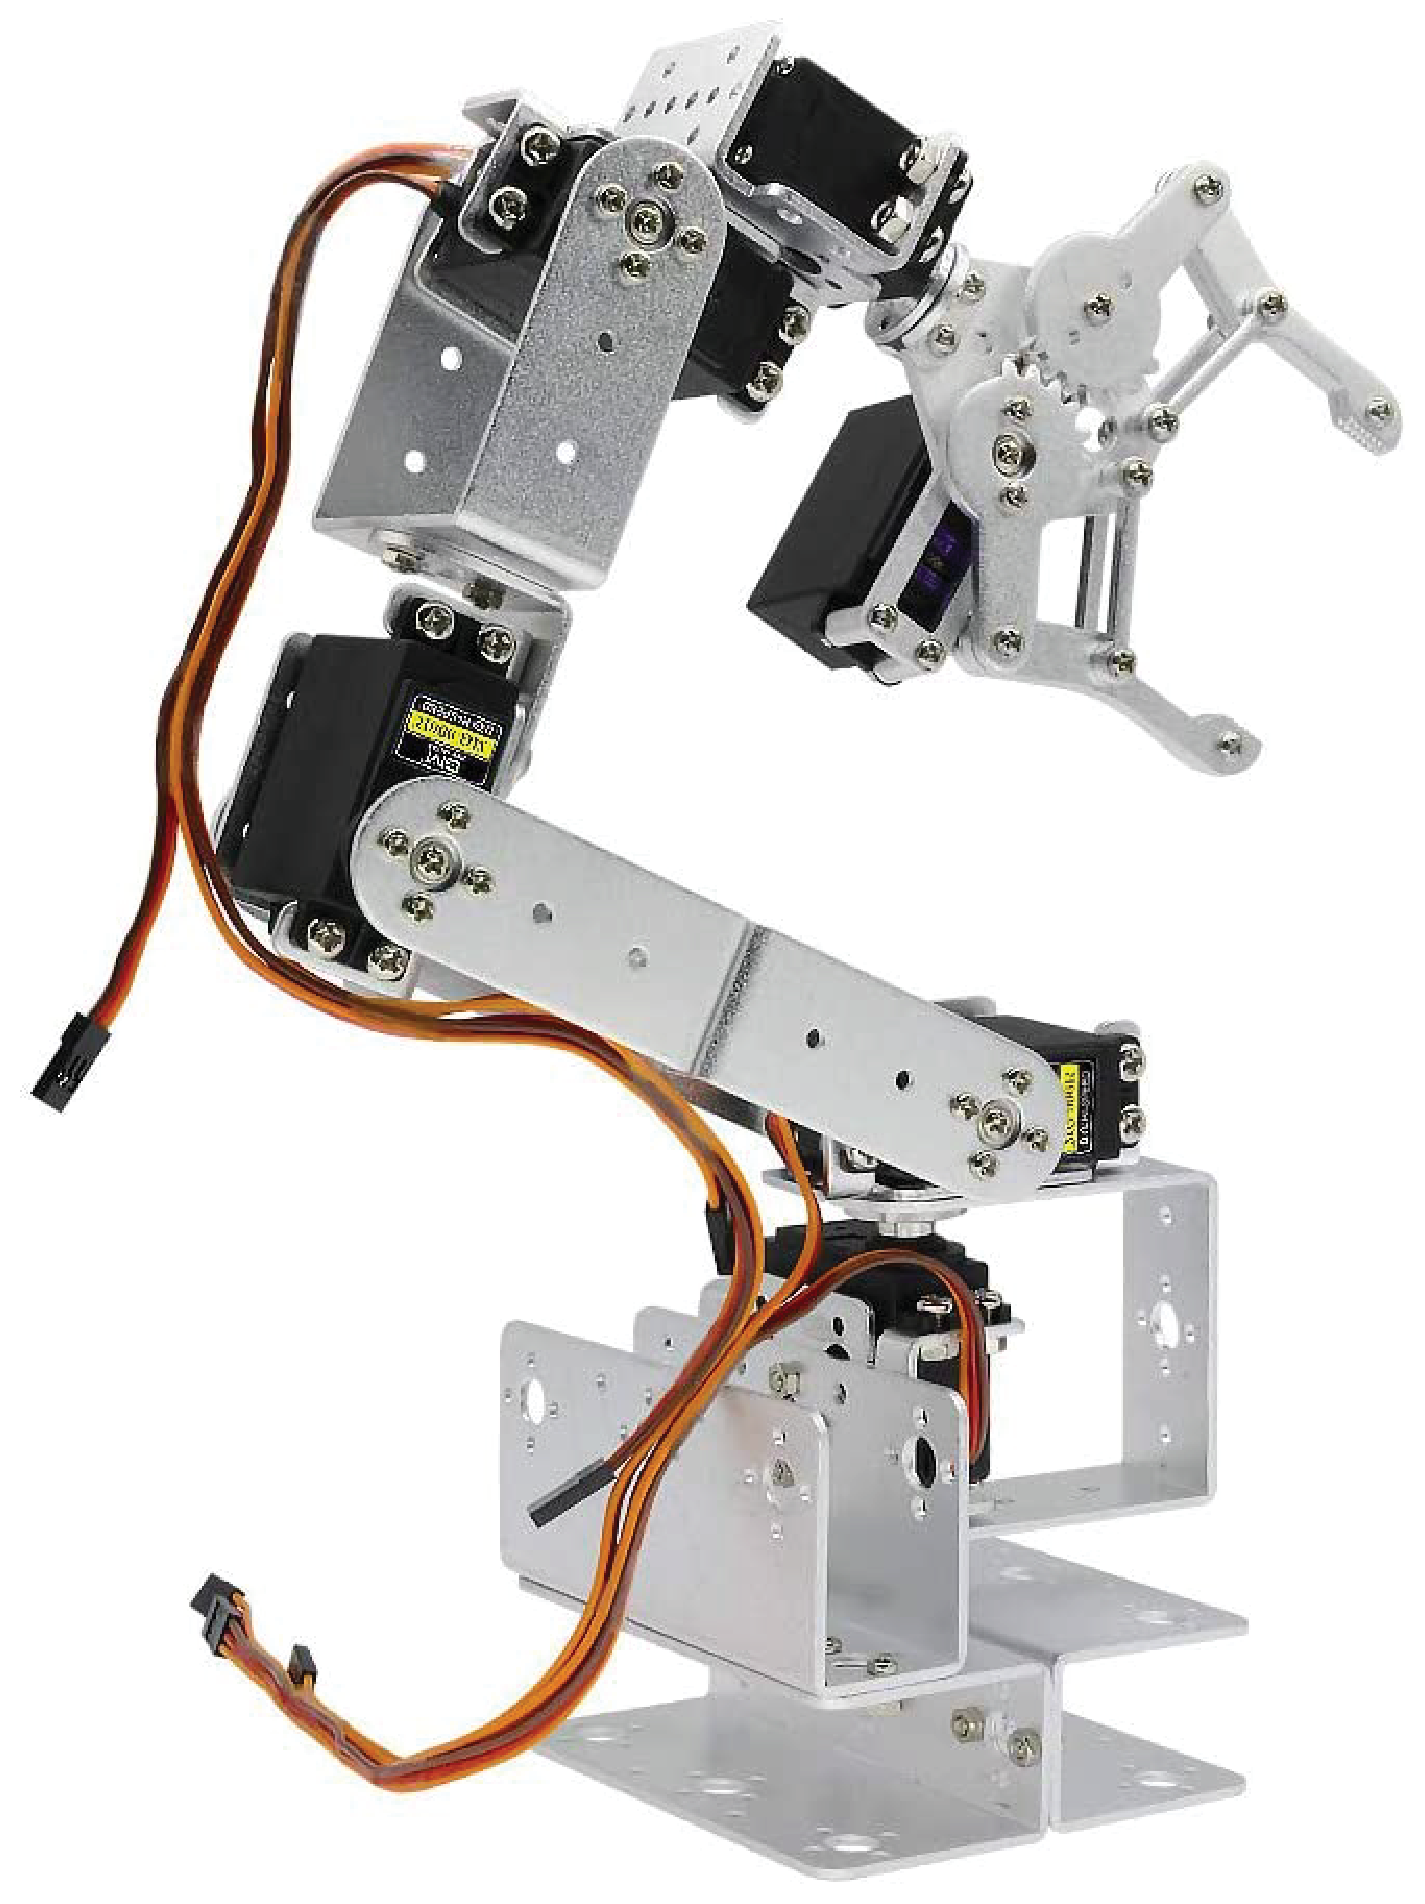
\includegraphics[scale=0.085]{robot_arm}
	%	\includegraphics[scale=0.08]{testbed_piborg}
	%	\includegraphics[scale=0.08]{testbed_robot_arm}
	%	\includegraphics[scale=0.09]{piborg_2_png}
	%	\includegraphics[scale=0.070]{robot_arm_2_png}
	\caption{Off-the-shelf testbeds: \ca multi-terrain rover (left) and \cb six-degree-of-freedom robotic arm (right).}
	\label{fig:demo_sys}
	\vspace*{-0.2\baselineskip}
\end{wrapfigure}


\paragraph{Demonstrative Platforms.} While our simulation-based studies focus on the scalability of the algorithms, we also aim to analyze the feasibility of our ideas in realistic environments. We will evaluate our ideas on \textit{two off-the-shelf cyber-physical platforms} (see Figure~\ref{fig:demo_sys}): \ca a multi-terrain ground rover (MonsterBorg~\cite{monsterborg}) and \cb a six-degree-of-freedom robotic arm (ROT3U~\cite{robot_arm_rot3u}). Our implementations will demonstrate the feasibility of security integration techniques on wide range of use-cases such as remote surveillance, home automation, and smart manufacturing. 

%We will use Raspberry Pi boards to control the hardware platforms and port our RT\_PREEMPT and LITMUS\textsuperscript{RT} scheduler plugins.  

%We will conduct both \textit{\ul{``blue team''} and \ul{``red team''} experiments }
%%to evaluate the efficacy of randomization protocols on our demonstrative platforms 
%where the red team will try to launch side-channel attacks on top of the defense mechanisms integrated by the blue team. The proposed setup will allow us to evaluate the efficacy of randomization protocols on real systems.









\section{Project Execution Plan}


Table~\ref{tab:timeline} presents the timeline of this project. The PI has already started mentoring the PhD student who would be supported by this project. 
%The students will be ideally prepared to work on the proposed research by the project start date. 
%The PI, along with graduate (and undergraduate) students, will meet once a week. 
The PI and students will meet at least once a week.
All students will congregate and jointly develop testbeds as well as work on the implementation. 
%The PI will also participate in \ca curriculum development — both, at the graduate and undergraduate levels and \cb outreach activities  throughout the project (see Section~\ref{sec:broader}). 
The PI will also participate in curriculum development and outreach activities  throughout the project (see Section~\ref{sec:broader}).
We will disseminate our research results from this work through scientific publications at \textit{top real-time conferences} (RTSS, RTAS, ECRTS) and \textit{multidisciplinary journals} (IEEE Access, IEEE TC), technical reports, open-source releases, prototype demonstrations/videos, and outreach activities.



\vspace{0.5em}
\begin{table}[!th]
%\begin{wraptable}{r}{9.50cm}
%	\vspace*{-0.5\baselineskip}
%	\begin{adjustbox}{width=01.00\textwidth}
%		\Huge
%		\scriptsize
		\small
		\centering
		\begin{tabular}{|l|l|l|l|l|l|l|l|l|}
			\hline
			\multicolumn{1}{|c|}{\multirow{3}{*}{\textbf{Description}}} & \multicolumn{8}{c|}{\textbf{Timeline}}                                                                        \\ \cline{2-9} 
			\multicolumn{1}{|c|}{}                                      & \multicolumn{4}{c|}{\textbf{Year 1}}                  & \multicolumn{4}{c|}{\textbf{Year 2}}                  \\ \cline{2-9} 
			\multicolumn{1}{|c|}{}                                      & \textbf{Q1} & \textbf{Q2} & \textbf{Q3} & \textbf{Q4} & \textbf{Q1} & \textbf{Q2} & \textbf{Q3} & \textbf{Q4} \\ \hline
			\textbf{TASK 1}: Design multi-mode security integration framework	&  \checkmark           & \checkmark             &             &             &             &             &             &             \\ \hline
			\textbf{TASK 2}: Support atomicity and task dependency &             &            & \checkmark            & \checkmark             &            &             &             &             \\ \hline
			\textbf{TASK 3}: Devise security metrics	&             &             &   \checkmark          &   \checkmark         &   \checkmark          &  \checkmark           &             &             \\ \hline
			\textbf{TASK 4}: Develop TrustZone-enabled monitoring framework &             &             &             &          \checkmark   & \checkmark            & \checkmark            & \checkmark              &             \\ \hline
			Testbed development and performance evaluation &             &       \checkmark      &  \checkmark           & \checkmark            & \checkmark            &  \checkmark           &  \checkmark           &  \checkmark           \\ \hline
			Education and outreach &   \checkmark          &  \checkmark           &   \checkmark          &     \checkmark        & \checkmark            &   \checkmark          &     \checkmark        &  \checkmark           \\ \hline
		\end{tabular}
		\caption{Timeline of our proposed research.}\label{tab:timeline}
%	\end{adjustbox}
	
%	\vspace*{-0.5\baselineskip}
%\end{wraptable}
\end{table}
%\vspace*{2mm}
\paragraph{Plans for Assessing Success.} We will evaluate our proposed research agendas based on the successful development of analytical models, performance metrics, and scheduler implementations.  We will also track the number of citations of our publications, monitor visits to our project website, and observe the number of downloads/forks of our public code repositories. We will measure the success of our education plans by monitoring the number of student enrollment, course evaluations, ratings/comments/feedback from the students, and successful completion of course projects that turn into research publications. Our assessment of outreach activities includes \ca monitoring the number of K-12 and undergraduate student participation and \cb successful development of new pedagogical contents. We will continuously monitor and evaluate our education and outreach activities and adjust them based on the observed results. 










% Header should be exactly this. 
%\section{Broader Impacts of the Proposed Work} \label{sec:broader}

\section{Broader Impacts} \label{sec:broader}




%\todo{fix.}


\paragraph{Societal Impact.} The proposed research and educational plans have the potential for broad impact. A large number of critical systems of modern society have real-time requirements (\eg avionics, automobiles, power grids, manufacturing plants, medical devices, industrial control systems, unmanned vehicles). They are also increasingly becoming targets for cyber attacks~\cite{stuxnet,Ukraine16,drone_threat2,dronhack,aircraft_hacking,checkoway2011comprehensive,koscher2010experimental,ddos_iot_camera,security_medical}. Any successful, profound attacks on these systems can have catastrophic results, leading to loss of injury to humans, negative impacts on the system and even the environment. Hence, techniques developed as part of this project will make such systems \textit{more secure} and applicable to a \textit{broad range of domains}. Our proposed research can lead to substantial improvements in consumer cyber-physical products and also improve systems that have \textit{national security considerations}. All data, insights, results, implemented frameworks, and course modules will be made available to the \textit{research community via a dedicated project website} along with appropriate documentation. Our public releases will facilitate the rapid dissemination and adoption of our ideas in the scientific community. 
%The proposed educational and outreach activities (described next) are expected to encourage underrepresented students to pursue careers in STEM.
In addition to technical contributions, our proposed educational and outreach activities (presented next) will have a broad and positive societal impact by \ca training a qualified workforce and \cb encouraging underrepresented students to pursue careers in computing.

\paragraph{Curriculum Development.} This proposal will feed into the PI's ongoing efforts to improve teaching real-time and cyber-physical systems, especially security concepts in these domains. 
%Students supported by this project will get a solid scientific foundation in designing and implementing real-time security solutions. Other students (not directly involved in the research) will also benefit through research seminars and scientific publications. 
The PI anticipates that the results obtained from this project will provide a foundation for \textit{one or more chapters in textbooks}. 

%Other students who are not directly involved in the project will also benefit through research seminars and scientific publications. 


 \textit{\textbf{$\diamond$~Development of a New Course:}} 
 
 
 \textit{\textbf{$\diamond$~Enhancement of Existing Courses:}} 
 



\paragraph{Diversity and Outreach.}

The PI is attentive to diversity and inclusion in his research and educational activities. 
%The PI strongly believes in maintaining a diverse research group and will make additional efforts to promote diversity.  
%While the PI make contributions towards educating all students, he will make additional efforts to promote diversity. 
The PI currently advises \textit{\ul{two female} graduate students} (one PhD and one MSc).
The proposal includes \textit{funding support for \ul{one female PhD student}} (Neha Chauhan) who has \textit{already started working on the project}. 
%One \textit{female PhD} (Neha Chauhan) is \textit{already working on the project}, and the budget of the proposal included two year funding support for her. 
%PI Hasan recruited another female PhD student 
%(Sara Yavari) 
%who will join from Fall'21. 
%The PI strongly believes in maintaining a diverse research group --- 
%The PI will \ca make additional efforts to promote equity, \cb recruit students from underrepresented communities, and  \cc  ensure that \textit{at least one position will be reserved all times for undeserved populations}. 
%The PI strongly believes in maintaining a diverse research group --- 
The PI will make additional efforts to promote diversity and  ensure that \textit{\ul{at least one position} will be reserved \ul{all times} in his research lab for underserved populations, including students with disabilities}. 


\textit{\textbf{$\diamond$~Broadening Participation in Wichita\footnote{Supporting letters from \textit{Ana Lazar\'in} (Director, Broadening Participation and Recruitment, College of Engineering), \textit{Vinod Namboodiri} (Wichita State REU program lead), and \textit{Joe Jabara} (Director, Hub for Cybersecurity Education and Awareness) are attached.}:}}  
%\textit{\textbf{$\diamond$~Broadening Participation in Wichita\footnote{Supporting letters are attached.}:}}  
The PI is working closely with Wichita State's Shocker Engineering Academy~\cite{wsu_sea} to increase the representation of minority communities in engineering. The program is supported by an NSF initiative called KS-LSAMP (Kansas Louis Stokes Alliances for Minority Participation). As a part of this program, the PI is currently mentoring \textit{\ul{two undergraduate students}} from underrepresented communities (including \textit{\ul{one black female}} student). The PI will continue this effort throughout this project. The PI will also offer projects for Research Experiences for Undergraduates (REU) program~\cite{wsu_netcps_reu} and provide research opportunities especially for \textit{freshman/sophomore undergraduate students} on topics related to security and resiliency of real-time systems. The proposed initiatives will provide research opportunities for undergraduate students from the very early stages of their academic careers. The PI is also actively involved in Wichita State Hub for Cybersecurity Education and Awareness (HCEA)~\cite{wsu_hcea}. As a part of this initiative, PI will organize \textit{CTF (capture the flag) competitions and security boot camps for middle and high school students} (Year 1 and Year 2, Summer semesters). The PI will also \textit{engage in a campaign} in Year 2 to attract under-represented groups using presentations by students from these communities.


 \textit{\textbf{$\diamond$~Other Outreach Activities:}} 
 The PI will \textit{mentor underrepresented students} by partnering with the CRA's Distributed Research Experiences for Undergraduates (DREU) program~\cite{cra_dreu}. The PI will apply to be a DREU faculty mentor at the beginning of the project and intends to mentor the students in both years.
The PI will also \textit{volunteer for presentations and demos} at events organized by government agencies such as NSA's CAE K12 CyberTalk~\cite{k12_cybertalk} throughout the project
to involve minority groups and high school seniors.

%
%\todo{shockers icorps?}
\section{Results from Prior NSF Support}

%The PI is a new faculty member --- 

%The PI has not received any grant or contract from any department, agency, or institution of the federal government.

The PI has not received any grant or contract from the federal government.

 





%%%%%%%%%%%%%%%%%%%%%%%%%%%%%%%%%%%%%%%
% E - REFERENCES CITED

\newpage
\pagenumbering{arabic}
\renewcommand{\thepage} {E--\arabic{page}}

\bibliographystyle{IEEEtran}
\bibliography{references_mh}


%%%%%%%%%%%%%%%%%%%%%%%%%%%%%%%%%%%%%%%
% F - BIOGRAPHICAL SKETCHES
% USE NSF APPROVED FILLABLE PDF



%%%%%%%%%%%%%%%%%%%%%%%%%%%%%%%%%%%%%%%
% G - BUDGET JUSTIFICATION

\newpage
\pagenumbering{arabic}
\renewcommand{\thepage} {G--\arabic{page}}
%\section*{\large \bf \hfill{}BUDGET JUSTIFICATION\hfill{} \\}

% NOTE: No more than 5 pages. [as of 2020]

Budget justification. 

%\includepdf[pages=-]{supplimentary_docs/Budget_Justification_210811.pdf}



%%%%%%%%%%%%%%%%%%%%%%%%%%%%%%%%%%%%%%%
% H - CURRENT AND PENDING SUPPORT
% USE NSF APPROVED FILLABLE PDF


%%%%%%%%%%%%%%%%%%%%%%%%%%%%%%%%%%%%%%%
% I - FACILITIES & RESOURCES

\newpage
\pagenumbering{arabic}
\renewcommand{\thepage} {I--\arabic{page}}
\section*{\large \bf \hfill{}FACILITIES, EQUIPMENT, AND OTHER RESOURCES\hfill{} \\}
% Describe any substantial collaboration with individuals not included in the budget; 
% should be documented in a letter of collaboration (unfunded collaboration)



\section*{FACILITIES}

%\paragraph{Department of Electrical Engineering and Computer Science.}

The PI is a faculty member in the department of Electrical Engineering and Computer Science (EECS). The proposed project leverages several computational infrastructures already in place at Wichita State University (WSU). The PI will utilize existing facilities, equipment, and resources to execute the proposed research successfully.

\vspace{0.5em}
\paragraph{Cyber-Physical Systems Security Research Lab.} 

The PI directs the Cyber-Physical Systems Security Research Lab (CPS2RL). This 800 square feet lab is located on WSU's main campus in Wallace Hall, Room 331. The proposed research activities will be conducted in this lab. The lab contains various evaluation platforms, including multiple embedded development boards (ZedBoard, Raspberry Pi, BeagleBone Black, and UP Extreme) running Linux operating systems, one FischerTechnik manufacturing testbed, and four 3D printers. The lab also includes four general-purpose workstations (2.4 GHz CPU, 8 GB RAM, and 256 GB solid-state hard drive) and necessary research spaces for graduate and undergraduate students. The students will use these development boards and workstations for simulations, prototype development, and experiments. The lab is available 24/7 for the PI and students.


\vspace{0.5em}
\paragraph{Office Spaces and Administrative Supports.} The PI has 100 square feet of private office space on WSU's main campus in Jabara Hall, Room 244. The office is appropriate for day-to-day activities and holding meetings for the project. The graduate and undergraduate students will have access to student cubicles in the PI's research lab (CPS2RL). The graduate students will also have access to student cubicles in Wallace Hall, Room 309. These offices are appropriate for the students' day-to-day scholarly activities required for the project. The PI and students also have secretarial and technical support services provided through their department.

\vspace{0.5em}
\paragraph{Outreach Activities.}
The PI will leverage WSU's existing outreach programs (\eg Shocker Engineering Academy, Research Experiences for Undergraduates program, and Security Education Hub) and work on broadening participation in computing (refer to the attached support letters). These resources are not included in the budget.



\vspace*{1em}
\section*{MAJOR EQUIPMENT}

Not applicable for this project.


\vspace*{1em}
\section*{OTHER RESOURCES}

\paragraph{Startup Support.} The PI has \$50,000 startup support. The PI will use \$3000 from his startup funds to purchase additional hardware (ground rover and robotic arm testbed) required for this project.

\vspace{0.5em}
\paragraph{General Resources.} The Office of research at WSU promotes the expertise of the faculty by facilitating all aspects of externally funded grants and contracts. 
%They provide oversight, assistance, and guidance to faculty for proposal preparation and the administration of awarded programs.
They will provide oversight, assistance, and guidance to administer this project once awarded.

\vspace{0.5em}
\paragraph{Other Computing/IT Resources.} 

WSU's high-performance computing cluster (BeoShock) has two large GPUs and 800 CPU cores. The cluster is available to the PI and students for large-scale simulations. All IT computing facilities are connected to the gigabit campus backbone. The PI and students have access to the computing facilities via Ethernet/Wireless connections. WSU also provides web spaces and dedicated URLs for hosting webpages. The university also provides video conferencing software (Zoom and Teams) that can be used to hold virtual meetings.





%%%%%%%%%%%%%%%%%%%%%%%%%%%%%%%%%%%%%%%
% J - DATA MANAGEMENT PLAN + POSTDOC MENTORING PLAN

\newpage
\pagenumbering{arabic}
\renewcommand{\thepage} {J--\arabic{page}}
\section*{\large \bf \hfill{}DATA MANAGEMENT PLAN\hfill{} \\}

% reset section counter
\setcounter{section}{0}
%\renewcommand*{\theHsection}{\the\value{section}}. % uncomment if hyperref is enabled



\section{Types of Data}


We will not use any data from other sources except those generated from our research activities. We expect the following data to be generated as a direct result of the work being proposed in this project: 
\vspace*{0.5em}
\begin{itemize}
	\item Algorithms, design documents, and code for proposed schemes.
	\item Metrics to analyze the effectiveness of security integration techniques and the evaluated values based on these metrics.
	\item Use cases and test harnesses for our implementations.
	\item Source code and documentation related to integrating security techniques in commodity operating systems (RT\_PREEMPT, LITMUS\textsuperscript{RT}, and OP-TEE).
	\item Analyses and evaluation tools such as simulation frameworks and the design of hardware testbeds (ground rover and robotic arm).
	\item Design of experiments, experimental results, analysis, and videos for demonstrations.
%	\item Reference designs for CSAW and F1TENTH competitions developed by undergraduate/graduate students.
	\item Reference designs for URCAF competition developed by undergraduate students.
	\item Student reports, project designs, software artifacts, and theses.
	\item Scientific publications with research findings.
	\item Course materials (\eg lecture notes, presentation slides, exams, and project assignments).
\end{itemize}




\vspace*{1em}
\section{Data and Metadata Standards}


All data will be electronic. We will utilize industry standards and publicly accepted data formats. The descriptions, algorithms, theories, results will be documented in conference and journal papers, technical reports, research notes, and online files.  Source files will be stored in appropriate formats for the specific applications. 
%For example, most of the operating system implementations will be developed in the C language and will be stored in \texttt{.c} and \texttt{.h} files. 
We will document source code in standard ways that indicate distribution license as well as source information. Data sets will be retained in their original form (binary, CSV, XML, JSON). Videos for demonstrations will be recorded in standard format (MP4). If the formats are not standardized, we will provide the relevant documentation of the data formats.

\vspace*{1em}
\section{Policies for Access and Sharing and Provisions for Appropriate Protection/Privacy}

The PI retains the right to use all data generated as part of this research and anticipates sharing of data through publications and open source releases. There will be no copyright or licensing issues associated with the data being collected and maintained. This study will only collect non-sensitive data. We will not collect any private data in this research and no personal identifiers will be recorded or retained by the PI or students. Hence, there will be no privacy concerns.

Any vulnerabilities in existing systems, if discovered, will be dealt with in the following manner: \ca we will actively work with the vendors to develop patches/safeguards that can mitigate the issues; \cb we will further provide 3--6 months of lead times to vendors in case they wish to work on the fix themselves.
The PI will only publish the results once these processes have been completed or lead times have lapsed.

\vspace*{1em}
\section{Policies and Provisions for Re-use, Re-distribution}

We will not enforce any permissions or restrictions on the released code and data as we hope to foster the open access initiatives. We will use popular open-source licenses such as Apache, BSD, GPL, and MIT for our released code. We will choose the specific license on a case-by-case basis depending on whether other open-source projects are used in the development.

\vspace*{1em}
\section{Plans for Archiving and Preservation of Access}

We will store initial code and data on computers/testbed machines where they are generated. We will periodically back up the data using versioning infrastructure (Git). Data will be archived on local servers/versioning websites (GitHub) and managed for long-term storage. 
%Our data will be encrypted with enterprise-grade data protection software. 
We will preserve the code and data and open access to them for at least five years after the award. After five years, we will continue to preserve the code and data through regular backups and maintenance on our lab's computers/local storage servers as well as on a public archiving website (GitHub).

\vspace*{1em}
\section{Policies for Dissemination and Sharing of Research Results}



%\section{Reproducibility, Access, and Sharing}
%\section{Dissemination/Sharing of Data}

%\paragraph{Reproducibility.}



%\paragraph{Reproducibility and Open Source Release.} 

The PI is attentive to the broad dissemination of his research findings. By preserving and making project data accessible, we will inform the broader community and foster discovery and collaboration. Several source code and findings from the PI's prior research efforts are publicly available on GitHub (\url{https://github.com/mnwrhsn}). The PI currently maintains a public GitHub repository for his research group (\url{https: //github.com/CPS2RL}). We will also create a dedicated website for this project under our departmental domain (\url{https://www.wichita.edu/academics/engineering/eecs/cps2rl/realtimesecurity}). We will provide contact information on the website to communicate with the PI directly. All data obtained from the research will be fully documented and publicly available on our project website and GitHub repositories. The documentation will describe our experimental settings, including how the experiments were conducted and how the data was measured. Our open-source releases will enable replication of the experiments by other researchers and practitioners. 

The PI and graduate students will internally participate in research seminars at the university to highlight the latest/preliminary results. We will broadly disseminate significant research findings through scholarly publications. For instance, algorithms, research methods, implementation details, and results will be disseminated via conference, journal, and workshop publications. Electronic manuscripts of publications will be available for public access on our project website. We will provide links to the appropriate publisher in case copyright issues prevent us from uploading the publications. Extended research results will be made available via technical reports on our project website and archived on our institutional repository (\url{https://soar.wichita.edu}). Videos recorded for demonstrations will be made available via public streaming sites such as YouTube, and access links will be provided on the project website.  
Course modules and lecture slides developed based on this work will be publicly available on our website. We will not release instructor resources (such as solutions to lab problems and homework assignments) on our website; however, they will be made available to educators upon request. 

All materials will contain an acknowledgment of NSF support as follows: \textit{``This material is based upon work supported by the National Science Foundation under Grant No. (NSF grant number).''} Additionally, we will include a disclaimer that \textit{``any opinions, findings, and conclusions or recommendations expressed in this material are those of the author(s) and do not necessarily reflect the views of the National Science Foundation.''} The PI will also work with the Wichita State University’s Office of Research to ensure that our activities conform to NSF's research dissemination and sharing policies/requirements.



\newpage
\section*{\large \bf \hfill{}POSTDOCTORAL MENTORING PLAN\hfill{} \\}

%Postdoctoral mentoring plan is not applicable to this proposal.
Not applicable for this proposal.




%%%%%%%%%%%%%%%%%%%%%%%%%%%%%%%%%%%%%%%
% K - COLLABORATORS
\newpage
\pagenumbering{arabic}
\renewcommand{\thepage} {K--\arabic{page}}
\section*{\large \bf \hfill{}COLLABORATORS AND OTHER AFFILIATIONS INFORMATION\hfill{} \\}

Not applicable for this proposal.


%%%%%%%%%%%%%%%%%%%%%%%%%%%%%%%%%%%%%%%
% ? - PERSONNEL
\newpage
\pagenumbering{arabic}
\renewcommand{\thepage} {\arabic{page}}
\section*{\large \bf \hfill{}PROJECT PERSONNEL AND PARTNER ORGANIZATIONS\hfill{} \\}
\vspace*{1em}
$\bullet$~~~Monowar Hasan; Wichita State University; PI


%%%%%%%%%%%%%%%%%%%%%%%%%%%%%%%%%%%%%%%
% SUPPORTING LETTERS


\end{document}
